\section{Design of initial implementation}\label{design}
Here we document the initial design for QuantEx. For separation of concerns we
divide QuantEx into three distinct layers as shown in figure \ref{fig:layers}.

\begin{figure}\label{fig:layers}
\centering
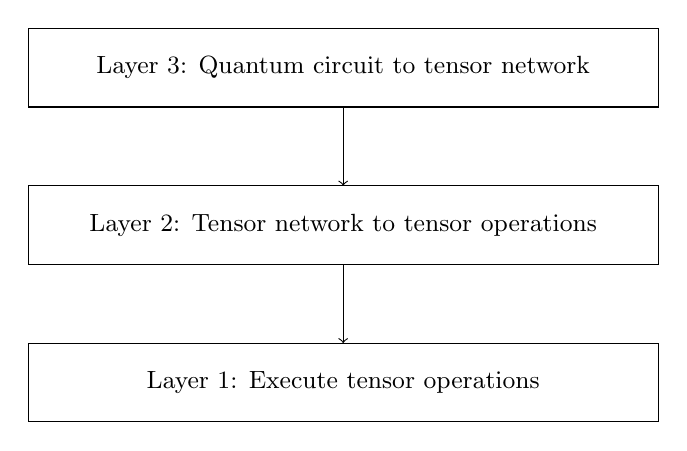
\begin{tikzpicture}
  \draw (0, 4) rectangle (8, 5);
  \node at (4, 4.5) {\small Layer 3: Quantum circuit to tensor network};
  \draw [->] (4, 4) -- (4, 3);

  \draw (0, 2) rectangle (8, 3);  
  \node at (4, 2.5) {\small Layer 2: Tensor network to tensor operations};
  \draw  [->] (4, 2) -- (4, 1);
    
  \draw (0, 0) rectangle (8, 1.0);
  \node at (4, 0.5) {\small Layer 1: Execute tensor operations};
\end{tikzpicture}
\caption{High level QuantEx architcture}
\end{figure}

\subsection{Layer 3: Quantum circuit to tensor network}
The highest level layer is responsible for converting an arbitrary quantum circuit to
a tensor network. The quantum assembly language (QASM) \cite{cross2017open}
is used as the format for describing quantum circuits. Using this open standard
format enables interoperability with the many available quantum computing
frameworks. We demonstrate each step here with an example circuit which
prepares a three qubit GHZ state. The circuit for preparing this state consists
of a Hadamard gate applied to the first qubit followed by controlled not gates
applied to the first and second and second and third qubits respectively. The
circuit is shown below and the QASM code describing this circuit is given in
listing \ref{lst:ghz_qasm}.

\begin{equation}\label{eqn:ghz_circuit}
    \Qcircuit @C=1.0em @R=0.0em @!R {
	 	\lstick{ q_{0} : \ket{0} } & \gate{H} & \ctrl{1} & \qw & \qw & \qw\\
	 	\lstick{ q_{1} : \ket{0} } & \qw & \targ & \ctrl{1} & \qw & \qw\\
	 	\lstick{ q_{2} : \ket{0} } & \qw & \qw & \targ & \qw & \qw\\
	 }
\end{equation}

\begin{minipage}{\linewidth}
\begin{lstlisting}[caption={QASM for three qubit GHZ preparation},label={lst:ghz_qasm}]
OPENQASM 2.0;
include "qelib1.inc";
qreg q[3];
h q[0];
cx q[0],q[1];
cx q[1],q[2];
\end{lstlisting}
\end{minipage}

\subsubsection{Tensor Network Notation and Conventions}
One of the trickier aspects of working with tensor networks is keeping track of
indices. Using graphical notation and maintaining consistency in how links
are labeled helps avoid confusion and prevent errors. Here we
present a short introduction to tensor networks, their graphical notation and
the index labeling conventions we will adopt for QuantEx. There are many
excellent resources for further reading on tensor networks and their use in
quantum information, for example see \cite{biamonte2017tensor, Bridgeman_2017, wood2011tensor}.

A tensor is a multi-dimensional array of numbers, where the rank gives the
number of dimensions. Graphically a tensor can be represented by a node with an
edge for each dimension. Figure \ref{fig:vector_matrix_tensors} shows how
vectors and matrices are represented graphically. Column vectors (or kets) have
an open link pointing to the right and row vectors (or bras) have an open link
pointing to the right.

An edge between tensors indicates contraction over the connected indices. Figure
\ref{fig:basic_tensor_contractions} shows how an inner product between two
vectors and a matrix vector multiplication are represented graphically. Using
this notation, we can represent quantum circuits graphically as tensor
networks. The three qubit GHZ preparation circuit shown in \ref{eqn:ghz_circuit}
can be represented as in figure \ref{fig:ghz_tn_circuit}.

\begin{figure}\label{fig:vector_matrix_tensors}
\centering
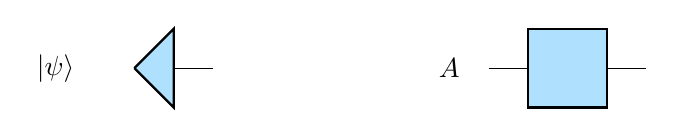
\begin{tikzpicture}
  \definecolor{lightblue}{RGB}{175,225,255}
  % draw vector and ket
  \node at (0, 0) {$|\psi\rangle$};
  \draw [black, fill=lightblue, thick] (1, 0) -- (1.5, 0.5) -- (1.5, -0.5) -- (1, 0);
  \draw (1.5, 0) -- (2, 0);
  
  % draw matrix
  \node at (5, 0) {$A$};
  \draw [black, fill=lightblue, thick] (6, -0.5) rectangle (7, 0.5);
  \draw (5.5, 0) -- (6, 0);
  \draw (7, 0) -- (7.5, 0);
\end{tikzpicture}
\caption{Graphical representation of vector and matrix}
\end{figure}

\begin{figure}\label{fig:basic_tensor_contractions}
\centering
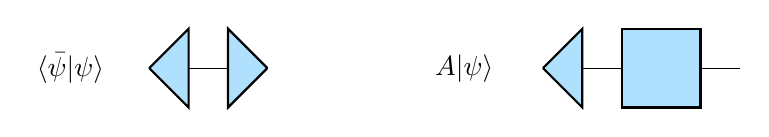
\begin{tikzpicture}
  \definecolor{lightblue}{RGB}{175,225,255}
  \node at (0, 0) {$\langle \bar{\psi} |\psi\rangle$};
  \draw [black, fill=lightblue, thick] (1, 0) -- (1.5, 0.5) -- (1.5, -0.5) -- (1, 0);
  \draw (1.5, 0) -- (2, 0);
  \draw [black, fill=lightblue, thick] (2.5, 0) -- (2, 0.5) -- (2, -0.5) -- (2.5, 0);
  
  \node at (5, 0) {$A | \psi \rangle $};
  \draw [black, fill=lightblue, thick] (6, 0) -- (6.5, 0.5) -- (6.5, -0.5) -- (6, 0);
  \draw [black, fill=lightblue, thick] (7, -0.5) rectangle (8, 0.5);
  \draw (6.5, 0) -- (7, 0);
  \draw (8, 0) -- (8.5, 0);
\end{tikzpicture}
\caption{Graphical representation of inner product and matrix vector multiplication}
\end{figure}

\begin{figure}\label{fig:ghz_tn_circuit}
\centering
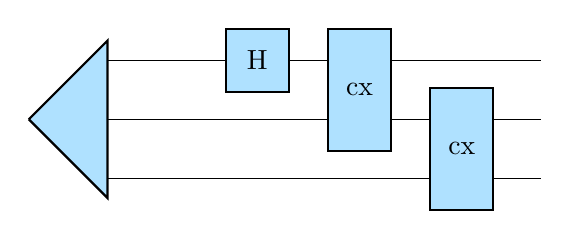
\begin{tikzpicture}
  \definecolor{lightblue}{RGB}{175,225,255}
  \draw [black, fill=lightblue, thick] (0, 0) -- (1, 1) -- (1, -1) -- (0, 0);
  \draw (1, 0.75) -- (2.5, 0.75);
  \draw [black, fill=lightblue, thick] (2.5, 0.35) rectangle (3.3, 1.15);
  \node at (2.9, 0.75) {H};
  \draw (3.3, 0.75) -- (3.8, 0.75);
  \draw (1, 0) -- (3.8, 0);
  \draw [black, fill=lightblue, thick] (3.8, -0.4) rectangle (4.6, 1.15);
  \node at (4.2, 0.375) {cx};
  \draw (4.6, 0.75) -- (6.5, 0.75);
  \draw (4.6, 0) -- (5.1, 0);
  \draw (1, -0.75) -- (5.1, -0.75);
  \draw [black, fill=lightblue, thick] (5.1, -1.15) rectangle (5.9, 0.4);
  \node at (5.5, -0.375) {cx};
  \draw (5.9, 0) -- (6.5, 0);
  \draw (5.9, -0.75) -- (6.5, -0.75);
\end{tikzpicture}
\caption{Three qubit GHZ preparation circuit as tensor network}
\end{figure}

The tensor network shown in figure \ref{fig:ghz_tn_circuit} does indeed
implement the GHZ circuit. However since the input state consists of a single
large tensor, storing this tensor requires the same amount of memory as full
wave-function methods. Breaking this large tensor into a network of smaller
tensors enables more compact representation of many states (maximally entangled
states require the same space as the full wave-function). Figure
\ref{fig:ghz_tn_mps_circuit} shows the same GHZ preparation circuit as in figure
\ref{fig:ghz_tn_circuit} but with the large input tensor broken into
individual tensors. In this case the large tensor is represented as a one
dimensional chain of tensors called a Matrix Product State (MPS). It is possible
to map the input tensor to other geometries including two or three dimensional arrays of tensors
with open/closed boundaries, fully connected networks of tensors or some
arbitrary graph. The geometry to map should be an input parameter to layer 3
with a sensible default if none is supplied. The use of the MPS representation has
particular benefits because it can be efficiently compressed
\cite{Schollw_ck_2011, zhou2020limits}.

\begin{figure}\label{fig:ghz_tn_mps_circuit}
\centering
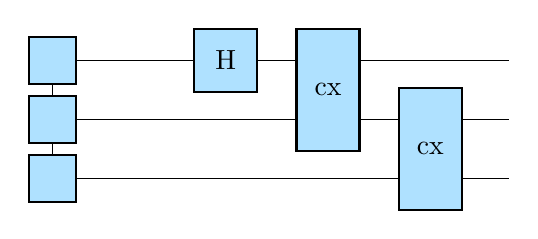
\begin{tikzpicture}
  \definecolor{lightblue}{RGB}{175,225,255}
  \draw [black, fill=lightblue, thick] (0.4, -0.3) rectangle (1.0, 0.3);
  \draw (0.7, 0.3) -- (0.7, 0.45);
  \draw [black, fill=lightblue, thick] (0.4, 0.45) rectangle (1.0, 1.05);
  \draw (0.7, -0.3) -- (0.7, -0.45);
  \draw [black, fill=lightblue, thick] (0.4, -1.05) rectangle (1.0, -0.45);
  \draw (1, 0.75) -- (2.5, 0.75);
  \draw [black, fill=lightblue, thick] (2.5, 0.35) rectangle (3.3, 1.15);
  \node at (2.9, 0.75) {H};
  \draw (3.3, 0.75) -- (3.8, 0.75);
  \draw (1, 0) -- (3.8, 0);
  \draw [black, fill=lightblue, thick] (3.8, -0.4) rectangle (4.6, 1.15);
  \node at (4.2, 0.375) {cx};
  \draw (4.6, 0.75) -- (6.5, 0.75);
  \draw (4.6, 0) -- (5.1, 0);
  \draw (1, -0.75) -- (5.1, -0.75);
  \draw [black, fill=lightblue, thick] (5.1, -1.15) rectangle (5.9, 0.4);
  \node at (5.5, -0.375) {cx};
  \draw (5.9, 0) -- (6.5, 0);
  \draw (5.9, -0.75) -- (6.5, -0.75);
\end{tikzpicture}
\caption{Three qubit GHZ preparation circuit as tensor network with a MPS used
  for the input state}
\end{figure}

\subsubsection{Tensor Network Internal Representation}

An internal representation for tensor networks is required for interchanging
tensor network descriptions between layers. Tensor networks are graphs where
nodes are tensors and edges contractions over tenor indices. For an interchange
format we require the ability to save the tensor data for each node along with
information on index ordering and edges. For this we build an internal graph
data structure and functionality convert to and from JSON format. The resulting 
JSON for a two qubit GHZ circuit is given in listing \ref{lst:ghz_json}.

\begin{lstlisting}[label=lst:ghz_json, basicstyle=\small, caption=Tensor network graph for two qubit GHZ circuit]
{
  "inputs": [
    1,
    2
  ],
  "outputs": [
    3,
    4
  ],
  "nodes": {
    "1": {
      "data_order": "col",
      "indices": [
        1
      ],
      "dims": [
        2
      ],
      "type": "input",
      "data_re": [
        1.0,
        0.0
      ],
      "data_im": [
        0.0,
        0.0
      ],
      "qubits": [
        1
      ]
    },
    "2": {
      "data_order": "col",
      "indices": [
        1
      ],
      "dims": [
        2
      ],
      "type": "input",
      "data_re": [
        1.0,
        0.0
      ],
      "data_im": [
        0.0,
        0.0
      ],
      "qubits": [
        2
      ]
    },
    "3": {
      "data_order": "col",
      "indices": [
        1
      ],
      "dims": [
        2
      ],
      "type": "output",
      "data_re": [
        1.0,
        0.0
      ],
      "data_im": [
        0.0,
        0.0
      ],
      "qubits": [
        3
      ]
    },
    "4": {
      "data_order": "col",
      "indices": [
        1
      ],
      "dims": [
        2
      ],
      "type": "output",
      "data_re": [
        1.0,
        0.0
      ],
      "data_im": [
        0.0,
        0.0
      ],
      "qubits": [
        4
      ]
    },
    "5": {
      "data_order": "col",
      "indices": [
        1,
        2
      ],
      "dims": [
        2,
        2
      ],
      "type": "gate",
      "data_re": [
        0.7071067811865475,
        0.7071067811865475,
        0.7071067811865475,
        -0.7071067811865475
      ],
      "data_im": [
        0.0,
        0.0,
        0.0,
        0.0
      ],
      "qubits": [
        0
      ]
    },
    "6": {
      "data_order": "col",
      "indices": [
        1,
        2,
        3,
        4
      ],
      "dims": [
        2,
        2,
        2,
        2
      ],
      "type": "gate",
      "data_re": [
        1.0,
        0.0,
        0.0,
        0.0,
        0.0,
        1.0,
        0.0,
        0.0,
        0.0,
        0.0,
        1.0,
        0.0,
        0.0,
        0.0,
        0.0,
        -1.0
      ],
      "data_im": [
        0.0,
        0.0,
        0.0,
        0.0,
        0.0,
        0.0,
        0.0,
        0.0,
        0.0,
        0.0,
        0.0,
        0.0,
        0.0,
        0.0,
        0.0,
        0.0
      ],
      "qubits": [
        0,
        1
      ]
    }
  },
  "edges": {
    "1": {
      "src": 1,
      "dst": 5,
      "indices": [
        1,
        1
      ]
    },
    "2": {
      "src": 2,
      "dst": 6,
      "indices": [
        1,
        2
      ]
    },
    "3": {
      "src": 5,
      "dst": 6,
      "indices": [
        2,
        1
      ]
    },
    "4": {
      "src": 6,
      "dst": 3,
      "indices": [
        3,
        1
      ]
    },
    "5": {
      "src": 6,
      "dst": 4,
      "indices": [
        4,
        1
      ]
    }
  }
}
\end{lstlisting}

\subsection{Layer 2: Tensor Network to Tensor Operations}


\subsection{Layer 1: Execute Tensor operations}